\section{Related Work}
%\subsection{Possible frameworks}
%There is a wide variety of web application frameworks. The PowerPedia prototype was build with the Recess PHP framework, but there are many %others, written in programming languages such as PHP, Ruby, Perl, or Java.  
%\subsection{Web platforms}
%\subsection{Energy feedback systems and community platforms}

There is a wide variety of web application frameworks. The PowerPedia prototype was build with the Recess PHP framework, but there are many others, written in programming languages such as PHP, Ruby, Perl, or Java.   
 
- welche frameworks kommen in frage?
- beispiele von web platformen, die diese framworks gebrauchen. 
- wieso wurden diese frameworks gebraucht?

\subsection{Collaborative web platforms}
The role of the user in modern web application is quite different from the pre Web 2.0~\footnote{Web 2.0 is a term introduced by Tim O'Reilly to describe a new generation of web applications~\cite{web2_0}} era. The web has become a collaborative medium, where users participate and collaborate to create content. Data is the driving force.

There are many examples of web platforms that build on collaboration. One of the most prominent ones is certainly Wikipedia~\footnote{\url{http://www.wikipedia.com}}, which only exists because of participating users. Wikipedia was launched in 2001 and consists of 19 millions articles, written by collaborators around the world~\cite{wikipedia}. Users have the possibility to create new articles or edit existing articles by extending and changing them, making improvement suggestions, or uploading multi media such as images. Wikipedia is run on the MediaWiki wiki software application~\footnote{\url{http://www.mediawiki.org}}. MediaWiki is written in PHP and was designed specifically for Wikipedia. 

Another area where users typically collaborate is software development. In a project where multiple developers work on the same code, a shared space for hosting and managing that code is needed. This is where hosting services such as Github~\footnote{https://github.com/} come into play. Github offers accounts for open source projects and uses the Git~\footnote{http://git-scm.com/} version control system.  

\subsection{Energy conservation platforms}
\subsubsection{Energy sensing}
\subsubsection{Collaborative energy conservation platforms}
\minisec{Energy conserving tips}
There exist various web platforms and sites to assist users in conserving energy. Especially websites with energy saving tips are quite numerous. Some of them encourage users to collaborate by offering the possibility to share their own energy saving ideas. The Swiss site of the World Wide Fund for Nature (WWF)~\cite{wwf} is a nice example. The focus is on using less resources in general, so electrical appliances is not the main focus, but of course an important topic as well. Users can rate tips, and give feedback if they are already following the advice or if they are willing to do so in the future. Every tip displays the number of users who checked either of the two options as well as the average rating. At the same time, there is a mobile phone application that lists electrical appliances that are especially energy efficient. Devices are sorted in device categories. For every category, there are tips when buying a new device, device category specific tips to conserve energy, and further information such as existing labels, publications and links to external sources. So far, there is no user collaboration in the mobile phone app. Additionally, tips and further information are displayed in a text document fashion, which make them tedious to read on a mobile phone. There is no "at one glance" overview and users have to do much scrolling to read the text.   

\minisec{Household level}
For Wattson~\footnote{DIY Kyoto. http://www.diykyoto.com/uk/wattson/about} owners, there is the possibility to become a member of the Wattson community~\footnote{http://community.diykyoto.com/members}. Registered users can download \textit{holmes}, a software that turns data collected by Wattson into plots and figures to illustrate how the the household uses electricity. From \textit{holmes}, measurement data can be uploaded to the community portal. The portal is a means to display the overall energy (in kWh), power and CO2 (number of tonnes of carbon dioxide released into the atmosphere as a result of the electricity used). Users can chose a time period and one of the above options and the website displays the corresponding figure. Further, the amount of money spent on electricity is displayed on the page, although this feature is not quite clear as there is no further description (see figure~\ref{wattson_community}). According to the documentation, users should be able to compare their consumption to that of other users, but it is unclear how to do that on the page. At the time accessed~\footnote{16.09.2011}, 2019 Wattson devices were connected to the portal. 
\begin{figure}[htbp]
\begin{center}
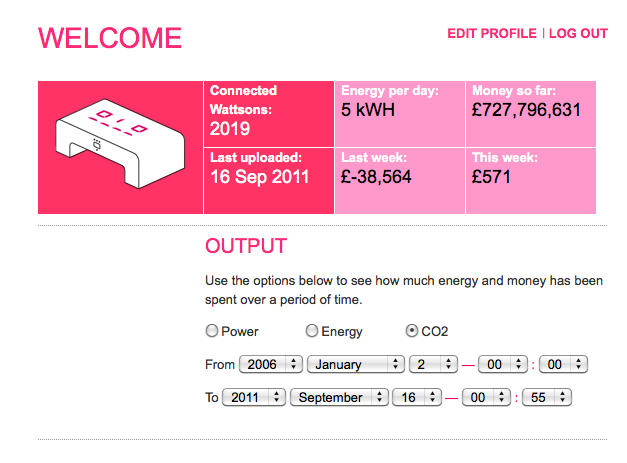
\includegraphics[width=6cm]{Images/wattson_community.png}
\caption{Wattson community portal}
\label{wattson_community}
\end{center}
\end{figure}

Another project, Velix~\footnote{\url{http://velix.vkw.at}}~\cite{energy_efficiency_online}, was developed by a group of researchers together with an Austrian electricity company. Velix provides users with feedback on their energy consumption and tips on how to save energy. The system aims at changing the users' behavior and daily routines. By giving users an overview over their energy consumption, users are supposed to get an idea of how much energy certain behaviors and routines need.  
Users are encouraged read their energy meter on a regular basis and publish the figures on the website on a weekly basis. Together with some general information about household size, heating method and house size, the energy efficiency of the user is calculated (see figure~\ref{velix}). 
In order to motivate a broader range of people to concern themselves with energy conservation, socio-psychological concepts were introduced in the project~\cite{improving_residential_energy_consumption}. Motivational elements such as rewards and commitment strategies help to keep users interested in the system. By uploading readings to Velix or fulfilling game-like tasks (such as signing up for a reminder to read the electricity meter, for example), points can be earned, which then can be exchanged for a real world gifts and prices.  
Velix was implemented with the open source content management system (CMS) Silverstripe~\footnote{http://www.silverstripe.com/}.
\todo{what kind of feedback is given to users?}  
  
\begin{figure}[htbp]
\begin{center}
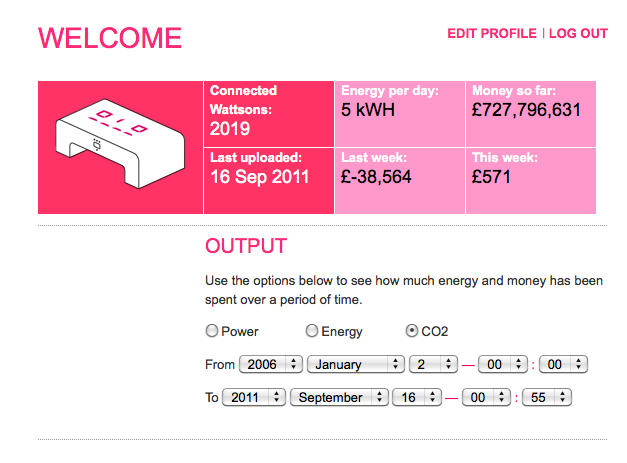
\includegraphics[width=6cm]{Images/wattson_community.png}
\caption{Wattson community portal}
\label{velix}
\end{center}
\end{figure}  
\minisec{Device level}  
On device level, the Energy Literacy Platform  (ELP)~\footnote{http://www.sassor.com/} is very promising idea. Unfortunately, the platform is only a prototype. The platform was proposed by the Japanese start up Sassor in 2010.
The proposed system consists of modules that can be plugged between the power plug and appliances, a receiver that collects the data from the different modules installed in the house, and the platform, which visualizes the measurements. The platform should display the consumption in real time (on both a device and household level), enable users to remotely switch on and off devices, compare values to friends and get energy saving tips.
Because there is no implementation yet, there are no further information on how data is compared or other details.